\section{Test numerowania}

Lorem ipsum dolor sit amet, consectetur adipiscing elit~\cite{test1}. Morbi sodales odio ac arcu facilisis sit amet ornare arcu rutrum~\cite{test1,test2}.

\begin{enumerate}
  \item{Cum sociis natoque penatibus et magnis dis parturient montes.}
  \item{Aliquam tincidunt urna.}
  \item{Nulla ullamcorper vestibulum turpis.}
\end{enumerate}

\lipsum[2]

\przyklad \lipsum[12] 

\noindent Aliquam porttitor quam a lacus (\emph{Rys.~\ref{fig:gfx-demo-1}}).


\begin{figure}[h!tb]
  \label{fig:gfx-demo-1}
  \centering
  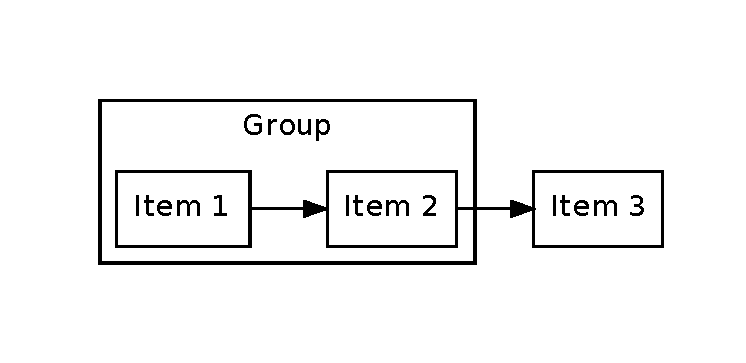
\includegraphics[width=.75\textwidth,trim={0 1cm 0 1cm}]{demo}
  \caption[Przykładowy rysunek]%
  {Przykładowy rysunek wygenerowany przez \emph{Graphviz}.}
\end{figure}

\subsection{Test podrozdziału}

\lipsum[3]

\begin{table}[h!tb]
  \center
  \caption{Przykładowa tabela}
  \label{my_table}
  \begin{tabular}{ | c | c | c | r | }
    \hline
  label 1 & label 2 & label 3 & label 4 \\
  \hline
  item 1  & item 2  & item 3  & item 4  \\
  \hline
  \end{tabular}
\end{table}

\lipsum[4]

\begin{figure}[h!tb]
  \centering
  
\includegraphics[width=5cm]{logo_pollub}
  \caption[Close up of \textit{Hemidactylus} sp.]%
  {Close up of \textit{Hemidactylus} sp., which is
  part the genus of the gecko family.}
\end{figure}

\lipsum[5]

\begin{table}[h!tb]
  \center
  \caption{Przykładowa tabela}
  \label{my_table}
  \begin{tabular}{ | c | c | c | r | }
    \hline
  label 1 & label 2 & label 3 & label 4 \\
  \hline
  item 1  & item 2  & item 3  & item 4  \\
  \hline
  \end{tabular}
\end{table}

\lipsum[6]

\begin{equation}
 \forall x \in X, \quad \exists y \leq \epsilon
\end{equation}

\lipsum[7]

\begin{equation}
 \forall x \in X, \quad \exists y \leq \epsilon
\end{equation}

\lipsum[8]

\cleardoublepage\thispagestyle{plain}
\section{Morbi laoreet nunc}

\lipsum[9]

\begin{figure}[h!tb]
  \centering
  
\includegraphics[width=4cm]{logo_pollub}
  \caption[Close up of \textit{Hemidactylus} sp.]%
  {Close up of \textit{Hemidactylus} sp., which is
  part the genus of the gecko family.}
\end{figure}

\lipsum[10]

\begin{lstlisting}[language=Python,caption={Przykładowy listing},label=lst:somelabel]
def create_search_result(request):
    query_type   = request.POST['type']
    query_string = request.POST['query'].strip().lower()
    query_id = get_result(query_type, query_string)

    return HttpResponseRedirect(reverse('show-search-result'))
\end{lstlisting}

\lipsum[11]


\begin{description}
  \item[Doneci]\hfill\\
    {Maecenas urna mi, suscipit in, placerat ut, vestibulum ut, massa. Fusce ultrices nulla et nisl.}
  \item[Aliquam]\hfill\\
    {\lipsum[15]}
  \item[Fusce]\hfill\\
    {\lipsum[14]}
\end{description}


\begin{table}[h!tb]
  \center
  \caption{Przykładowa tabela}
  \label{my_table}
  \begin{tabular}{ | c | c | c | r | }
    \hline
  label 1 & label 2 & label 3 & label 4 \\
  \hline
  item 1  & item 2  & item 3  & item 4  \\
  \hline
  \end{tabular}
\end{table}

\lipsum[12]

\begin{equation}
 \forall x \in X, \quad \exists y \leq \epsilon
\end{equation}

\lipsum[13]
